\documentclass[11pt]{article}
\usepackage[T1]{fontenc}
\usepackage{lmodern}
\usepackage{parskip}
\usepackage[colorlinks=true,urlcolor=Blue,linkcolor=black,citecolor=black]{hyperref}
\usepackage{graphicx}
\usepackage{amsmath}
\usepackage[utf8]{inputenc}
\usepackage[spanish]{babel}
\usepackage{fancyhdr}
\usepackage{csquotes}
\usepackage{lastpage}
\usepackage{array}
\usepackage{listings}
\usepackage{color}
\definecolor{dkgreen}{rgb}{0,0.6,0}
\definecolor{gray}{rgb}{0.5,0.5,0.5}
\definecolor{mauve}{rgb}{0.58,0,0.82}
\usepackage[affil-it]{authblk}
\usepackage[activate={true,nocompatibility},final,tracking=true,kerning=true,spacing=true,factor=1100,stretch=10,shrink=10]{microtype}
\usepackage[hmargin=2cm,top=4cm,headheight=65pt,footskip=65pt]{geometry}
\usepackage{hyperref}
\usepackage{graphicx}
\usepackage{float}
\usepackage{tabularx}
\graphicspath{ {./screenshots/p04/} }

% Documento
\begin{document}

% Título
\title{IFA. Práctica de laboratorio 04}

\author{Hugo Fonseca Díaz \\ email \href{mailto:uo258318@uniovi.es}{uo258318@uniovi.es}}
\affil{Escuela de Ingeniería Informática. Universidad de Oviedo.}

\maketitle

% Ejercicio 1
\section{Ejercicio 1}
Se crea el caso en Autopsy con los datos solicitados.

\begin{figure}[H]
    \caption{Ejercicio 1: Creación del caso}
    \centering
    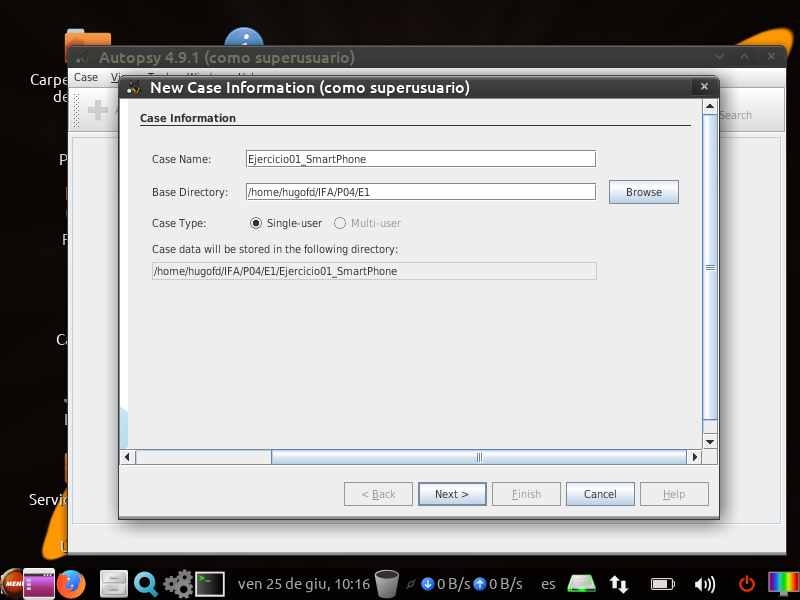
\includegraphics[scale=0.7]{e1-1.png}
\end{figure}

\begin{figure}[H]
    \caption{Ejercicio 1: Detalles del examinador}
    \centering
    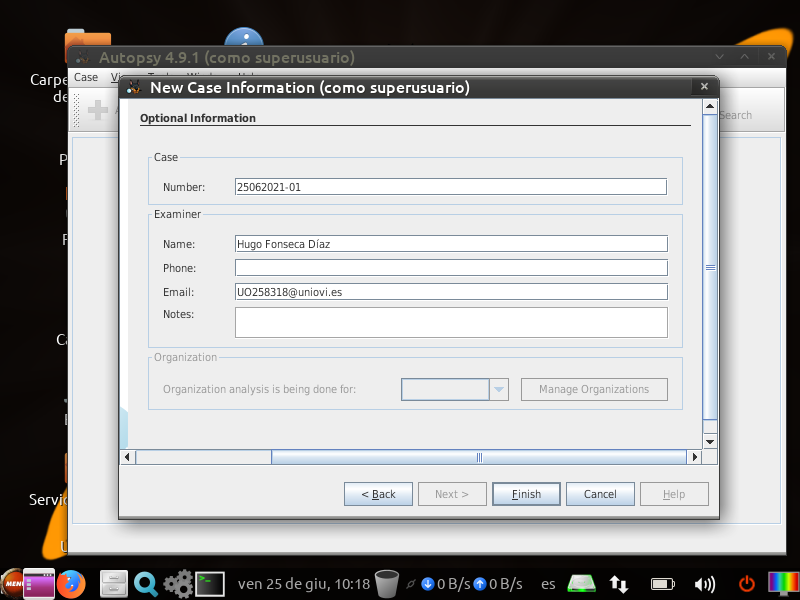
\includegraphics[scale=0.7]{e1-2.png}
\end{figure}

Añadimos la imagen a analizar.

\begin{figure}[H]
    \caption{Ejercicio 1: Selección de la imagen}
    \centering
    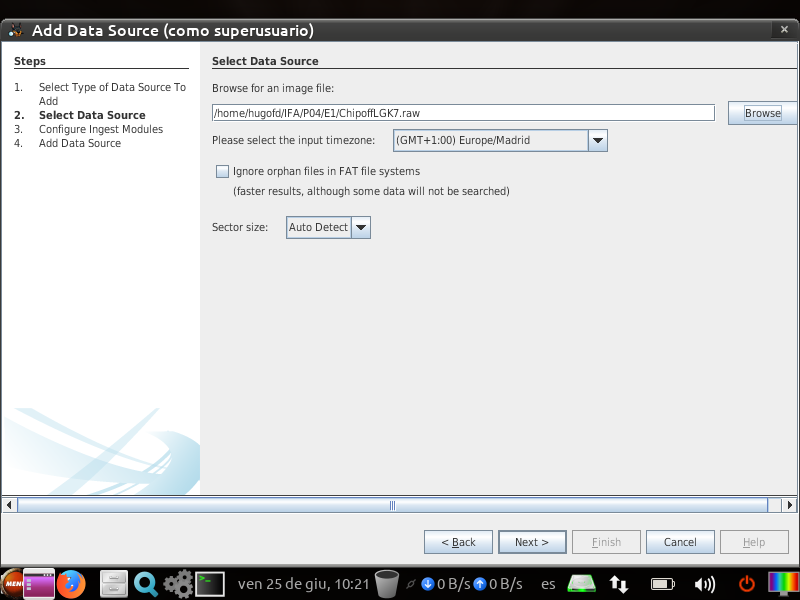
\includegraphics[scale=0.7]{e1-3.png}
\end{figure}

Se ejecutan los módulos de uno en uno para que el cómputo no sea excesivo. El que más tarda en ejecutarse es el módulo de búsqueda de palabras clave, el cual se ha dejado para el final.

\begin{figure}[H]
    \caption{Ejercicio 1: Ejecución del módulo de búsqueda de palabras clave}
    \centering
    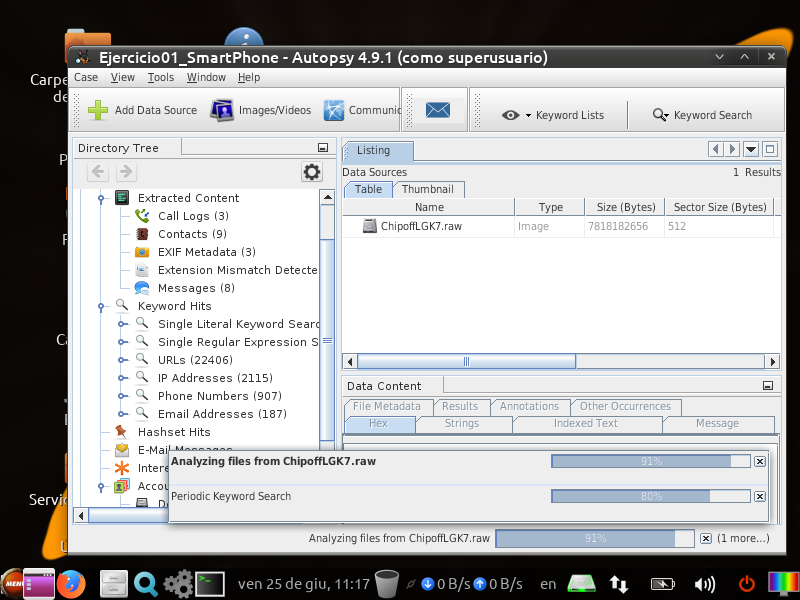
\includegraphics[scale=0.7]{e1-4.png}
\end{figure}

Una vez finalizada la ejecución de los módulos, se tienen los datos necesarios para responder a las cuestiones del ejercicio.

\begin{figure}[H]
    \caption{Ejercicio 1: Resultados del análisis}
    \centering
    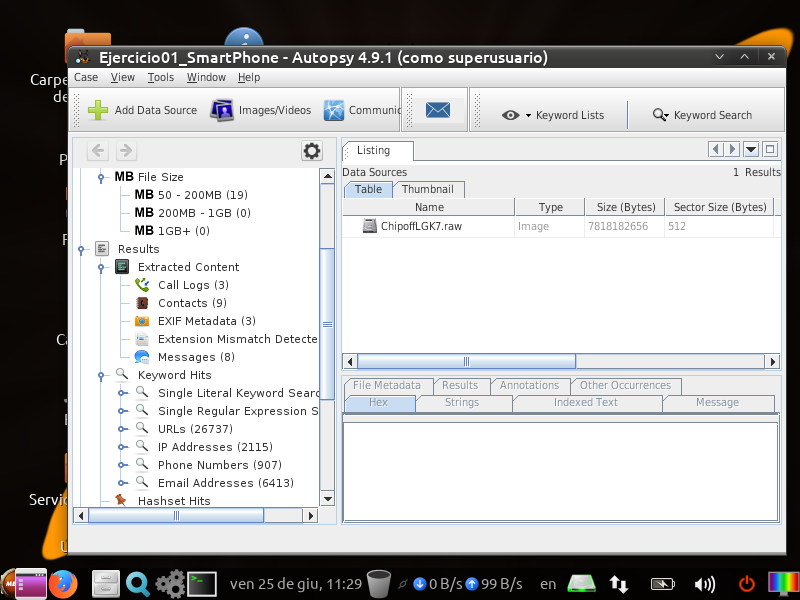
\includegraphics[scale=0.7]{e1-5.png}
\end{figure}

a) Como se puede observar en la siguiente imagen, hay un total de 9 entradas en el apartado de contactos.

\begin{figure}[H]
    \caption{Ejercicio 1: Contactos}
    \centering
    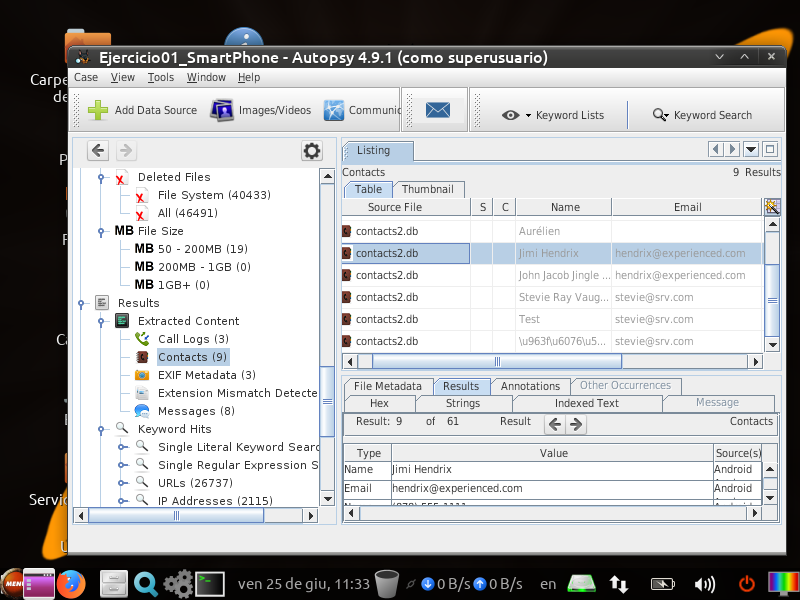
\includegraphics[scale=0.7]{e1-6.png}
\end{figure}

b) Jimi Hendrix, como se puede ver en la siguiente captura.

\begin{figure}[H]
    \caption{Ejercicio 1: Jimi Hendrix}
    \centering
    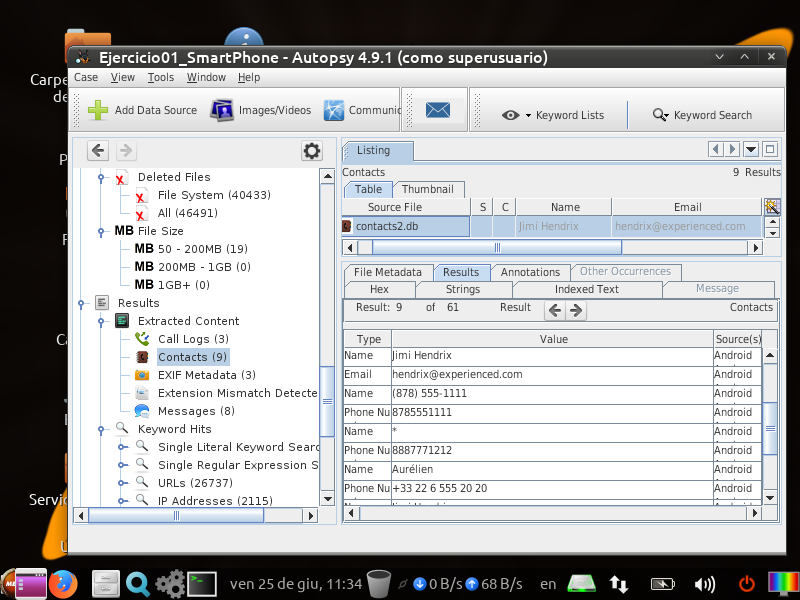
\includegraphics[scale=0.7]{e1-7.png}
\end{figure}

c) \textit{hendrix@experienced.com}, como se puede observar en la anterior captura.

d) El correo aparece dos veces, cada vez con un número distinto, pero si se tiene en cuenta el nombre del contacto, 7691234560.

\begin{figure}[H]
    \caption{Ejercicio 1: Teléfono de Jimi Hendrix}
    \centering
    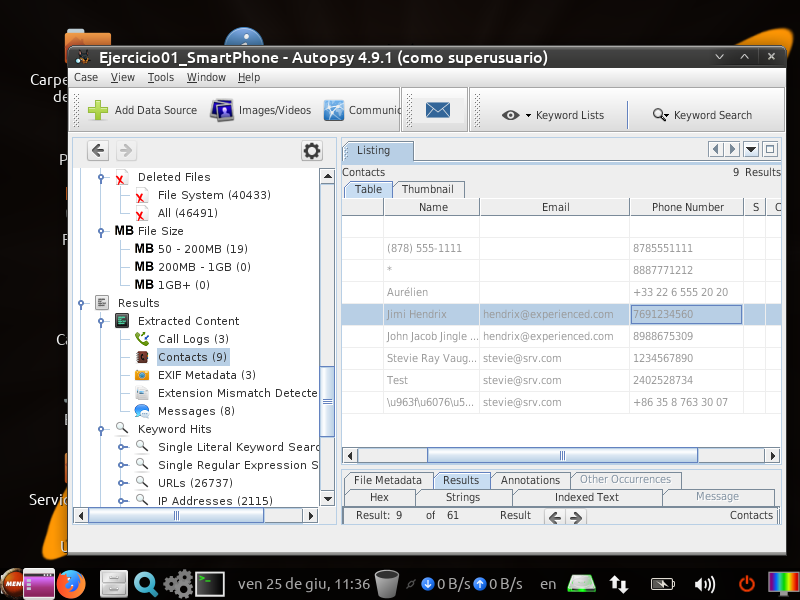
\includegraphics[scale=0.7]{e1-8.png}
\end{figure}

e) Hay una llamada saliente.

\begin{figure}[H]
    \caption{Ejercicio 1: Logs de llamadas}
    \centering
    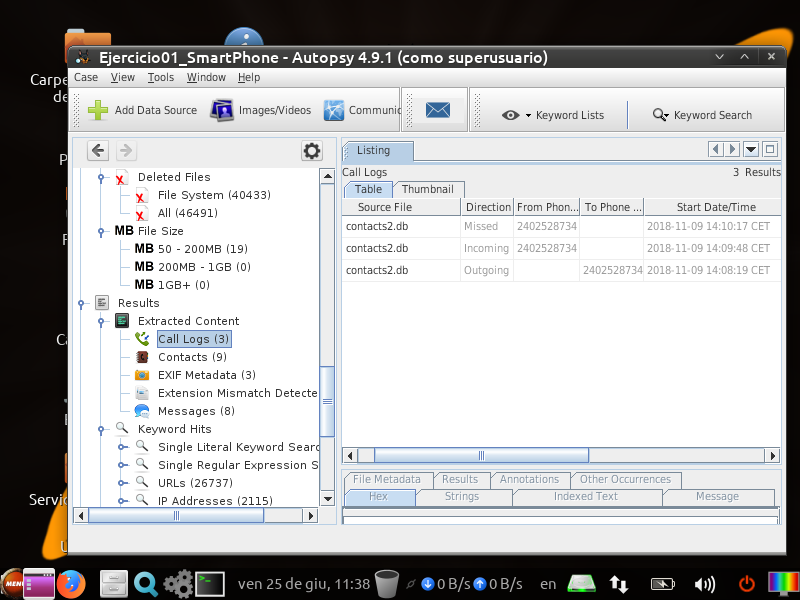
\includegraphics[scale=0.7]{e1-9.png}
\end{figure}

f) Del teléfono analizado al número de teléfono 2402528734.

g) Tres ficheros.

\begin{figure}[H]
    \caption{Ejercicio 1: Metadatos EXIF}
    \centering
    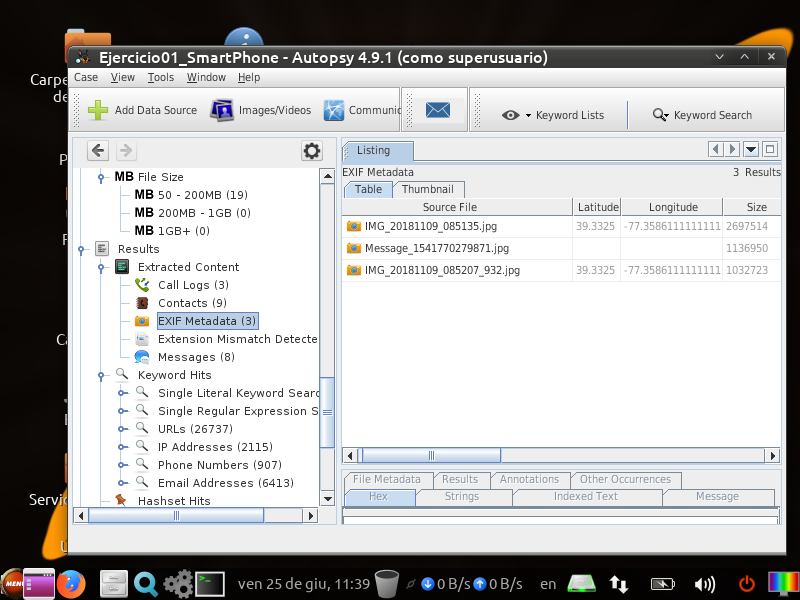
\includegraphics[scale=0.7]{e1-10.png}
\end{figure}

h) Dos de ellos tienen longitud y latitud (y uno de esos dos altitud). El tercero solo tiene la altitud. 

\begin{figure}[H]
    \caption{Ejercicio 1: Metadatos de coordenadas}
    \centering
    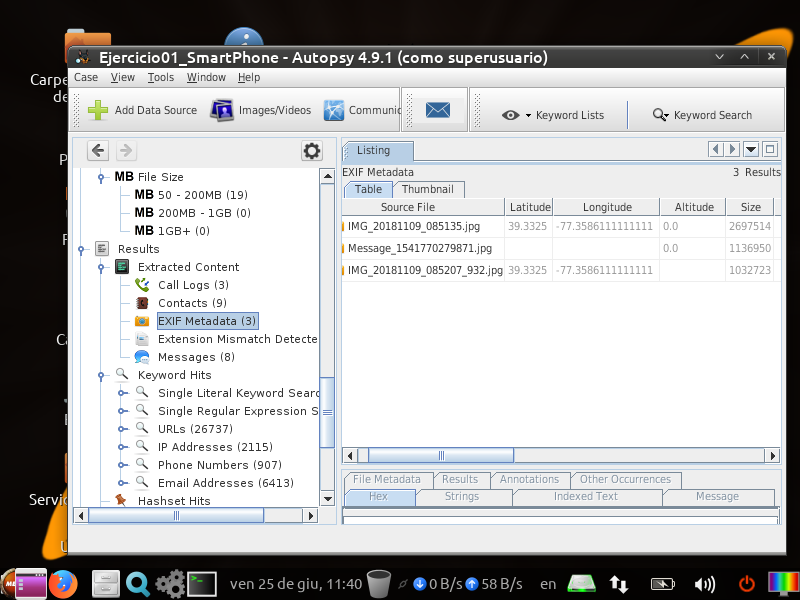
\includegraphics[scale=0.7]{e1-11.png}
\end{figure}

i) TBD GOOGLE MAPS

j) TBD GOOGLE MAPS

k) Con la cámara LGMS330 de un dispositivo LG.

\begin{figure}[H]
    \caption{Ejercicio 1: Modelo de cámara}
    \centering
    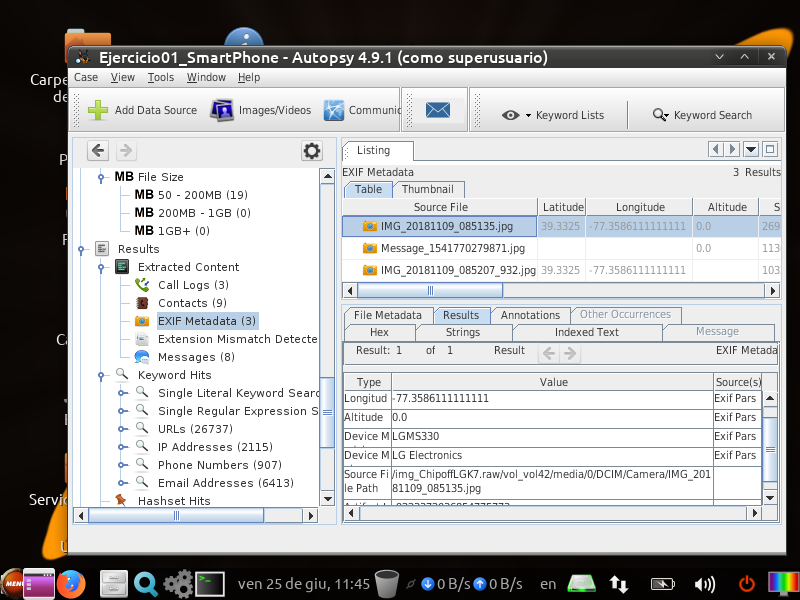
\includegraphics[scale=0.7]{e1-12.png}
\end{figure}

l) 2018/11/09 08:51:35

\begin{figure}[H]
    \caption{Ejercicio 1: Información de la imagen}
    \centering
    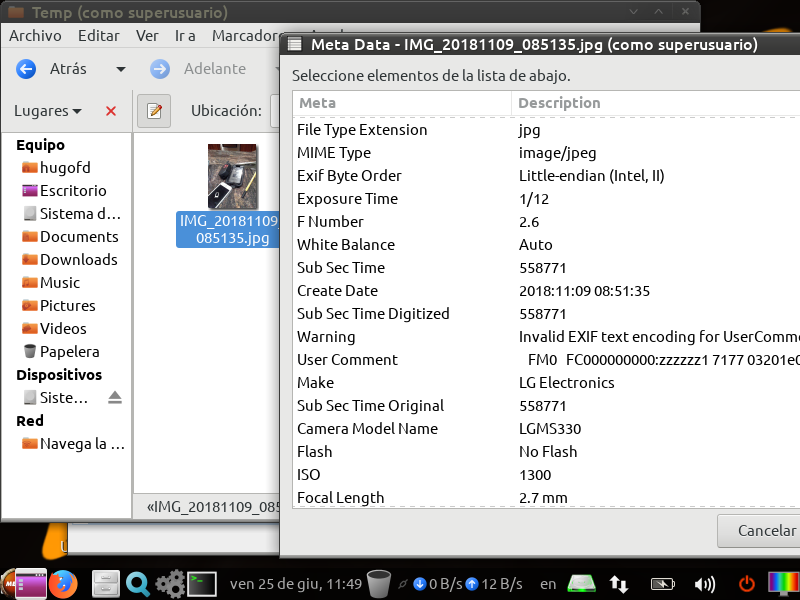
\includegraphics[scale=0.7]{e1-13.png}
\end{figure}

m) 2018/11/09 13:51:36

\begin{figure}[H]
    \caption{Ejercicio 1: Fecha de creación de la imagen}
    \centering
    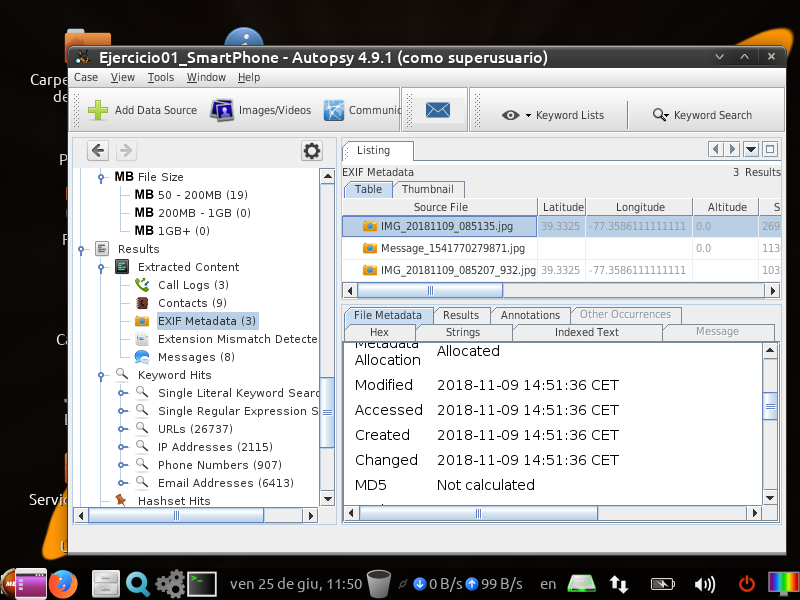
\includegraphics[scale=0.7]{e1-14.png}
\end{figure}

n) No, hay diferencias entre la hora de modificación del inodo y del fichero y la hora de creación y de acceso del fichero.

\begin{figure}[H]
    \caption{Ejercicio 1: MAC times}
    \centering
    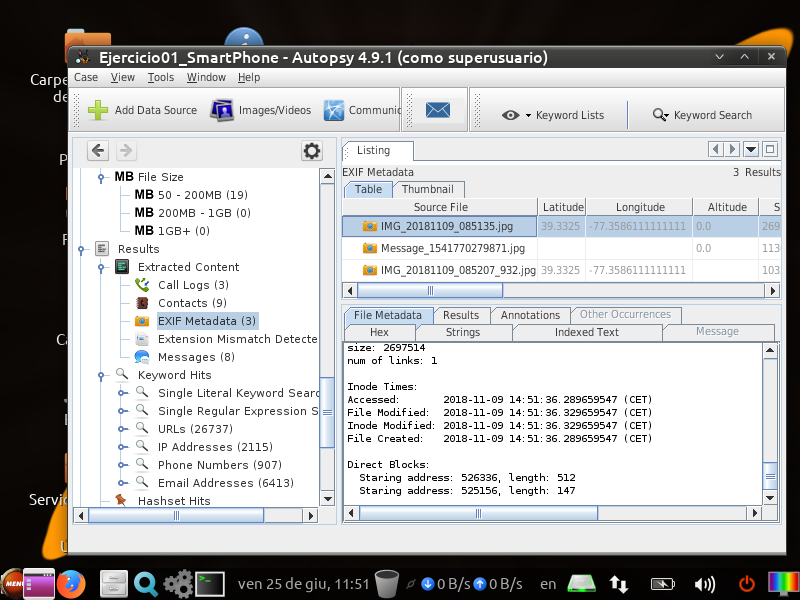
\includegraphics[scale=0.7]{e1-15.png}
\end{figure}

o) Hay dos móviles, uno de color blanco y otro oscuro con funda negra.

\begin{figure}[H]
    \caption{Ejercicio 1: Foto móviles}
    \centering
    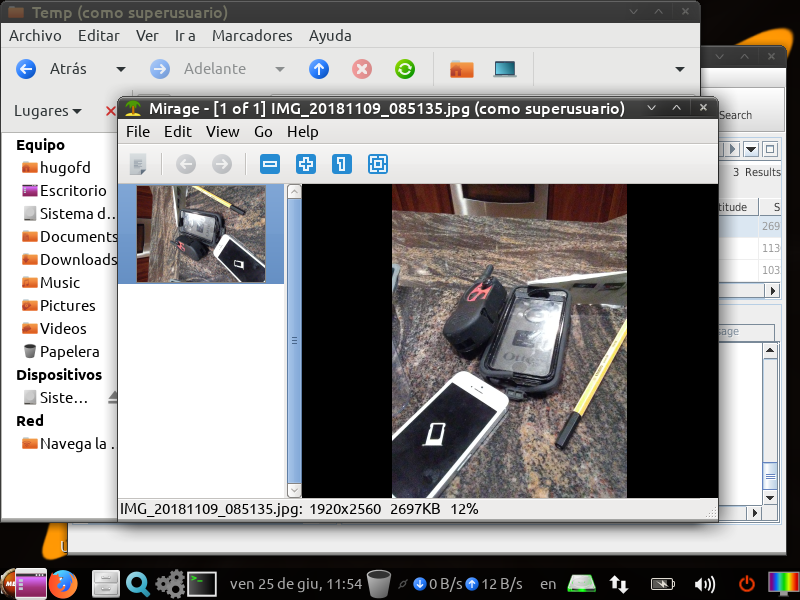
\includegraphics[scale=0.7]{e1-16.png}
\end{figure}

p) Se puede ver en la captura anterior, 1920x2560.

q) Una velocidad de obturación de 1/12.

\begin{figure}[H]
    \caption{Ejercicio 1: Velocidad de obturación}
    \centering
    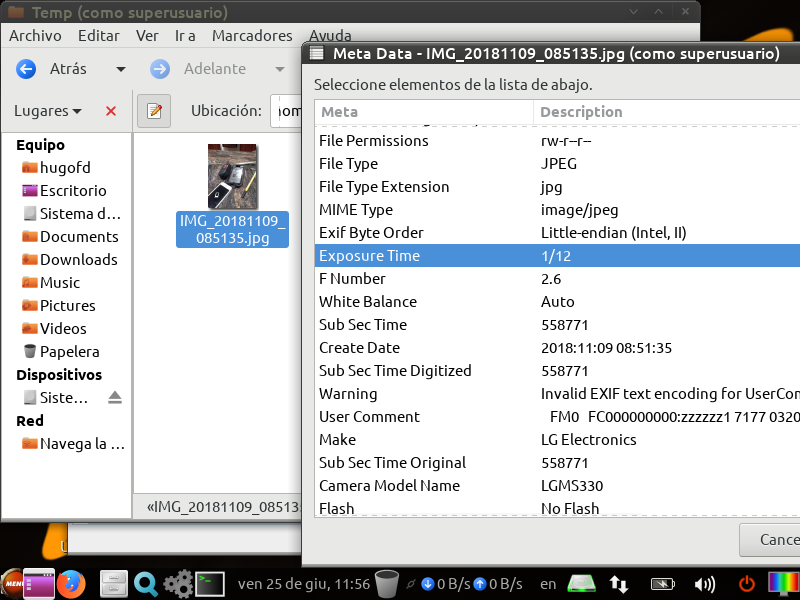
\includegraphics[scale=0.7]{e1-17.png}
\end{figure}

r) No se utilizó flash.

\begin{figure}[H]
    \caption{Ejercicio 1: No flash}
    \centering
    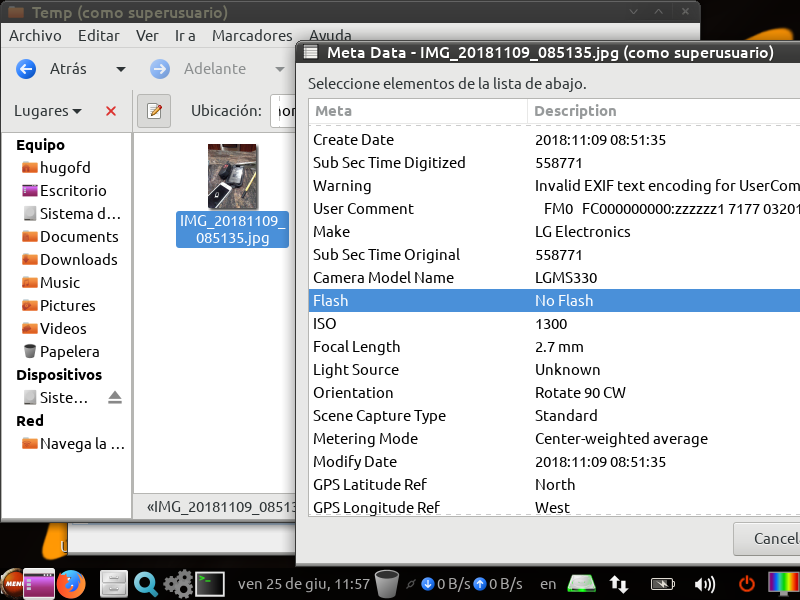
\includegraphics[scale=0.7]{e1-18.png}
\end{figure}

s) Hay un fichero \textit{emma-girl.jpg}.

\begin{figure}[H]
    \caption{Ejercicio 1: Carpeta download}
    \centering
    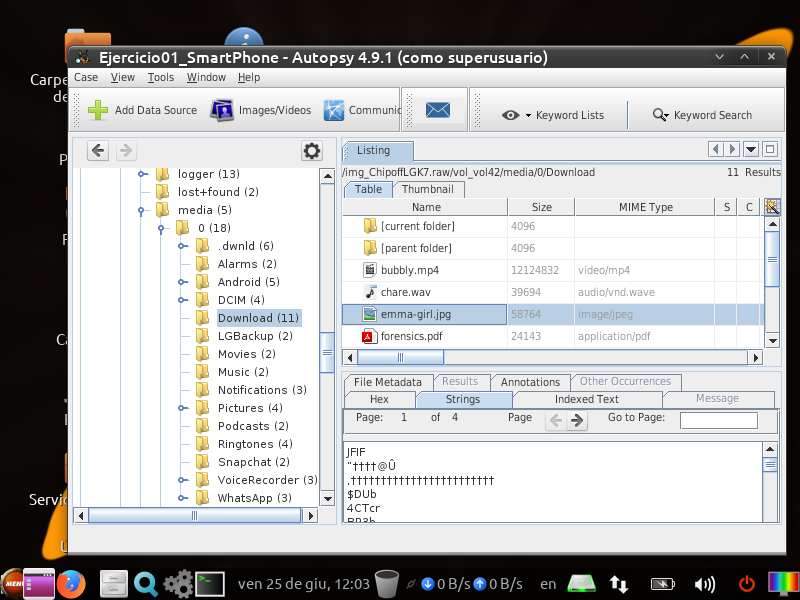
\includegraphics[scale=0.7]{e1-20.png}
\end{figure}

\begin{figure}[H]
    \caption{Ejercicio 1: \textit{emma-girl.jpg}}
    \centering
    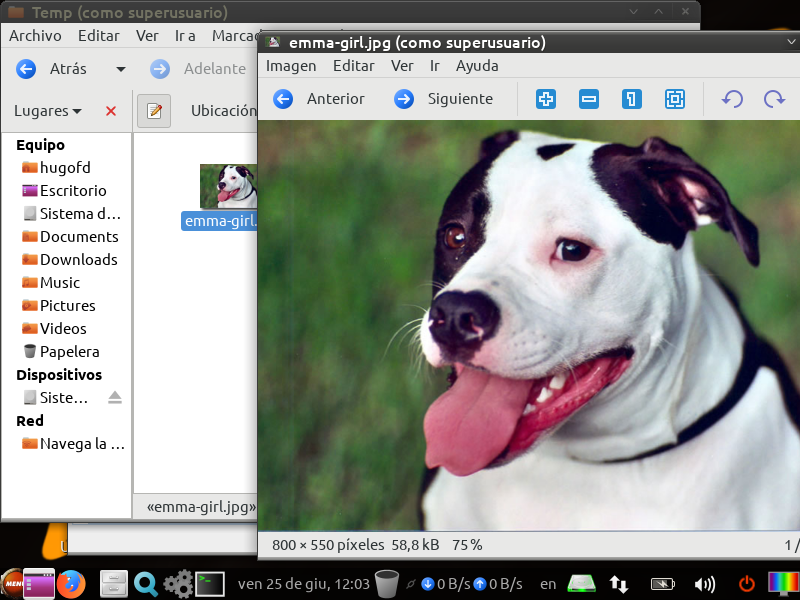
\includegraphics[scale=0.7]{e1-19.png}
\end{figure}

t) Uno, llamado \textit{forensics.pdf}.

\begin{figure}[H]
    \caption{Ejercicio 1: Carpeta download (de nuevo)}
    \centering
    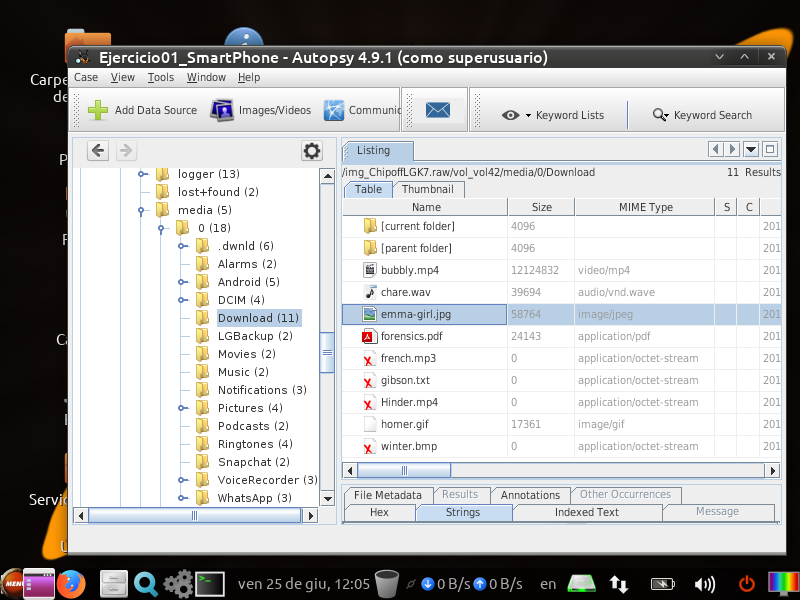
\includegraphics[scale=0.7]{e1-21.png}
\end{figure}

u) Cuatro, como se ve en la anterior captura.

v) En la carpeta download hay un fichero pdf llamado \textit{forensics.pdf}.

w) Se muestra su contenido en la siguiente captura.

\begin{figure}[H]
    \caption{Ejercicio 1: \textit{forensics.pdf}}
    \centering
    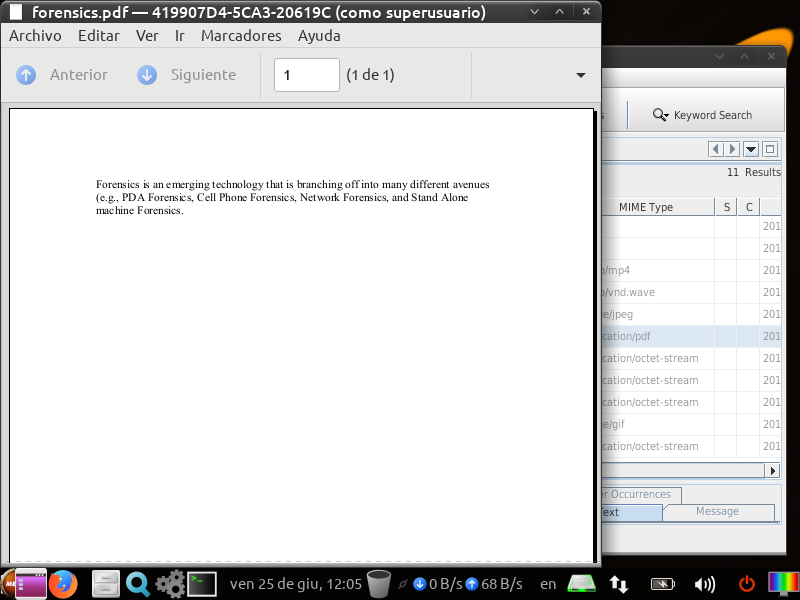
\includegraphics[scale=0.7]{e1-22.png}
\end{figure}

x) Los mensajes pueden encontrarse en Extracted Content, Messages. El mensaje con el código de Whatsapp se muestra a continuación.

\begin{figure}[H]
    \caption{Ejercicio 1: Mensaje con el código de Whatsapp}
    \centering
    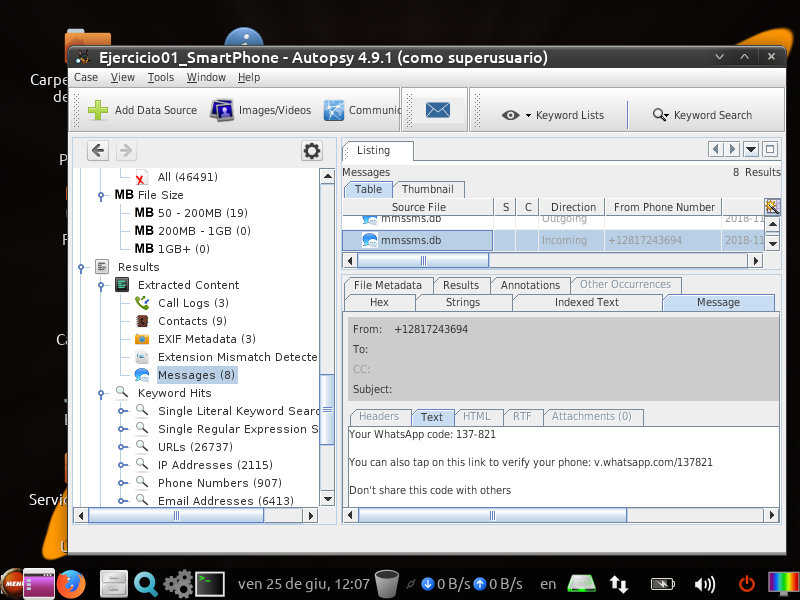
\includegraphics[scale=0.7]{e1-23.png}
\end{figure}

y) El mensaje aparece como \textit{No leído}.

\begin{figure}[H]
    \caption{Ejercicio 1: No leído}
    \centering
    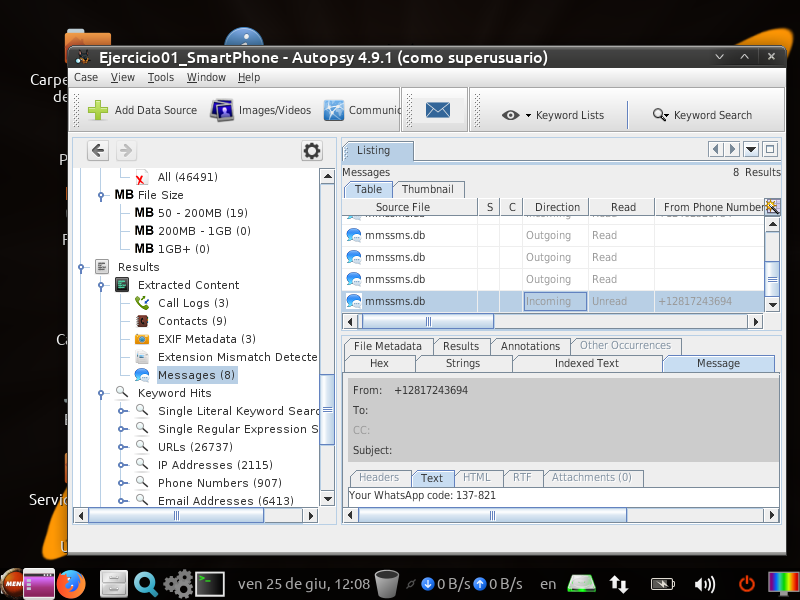
\includegraphics[scale=0.7]{e1-24.png}
\end{figure}

z) El mensaje se recibió el 2018/11/09 a las 14:47:35 CET.

\begin{figure}[H]
    \caption{Ejercicio 1: Fecha y hora de recepción}
    \centering
    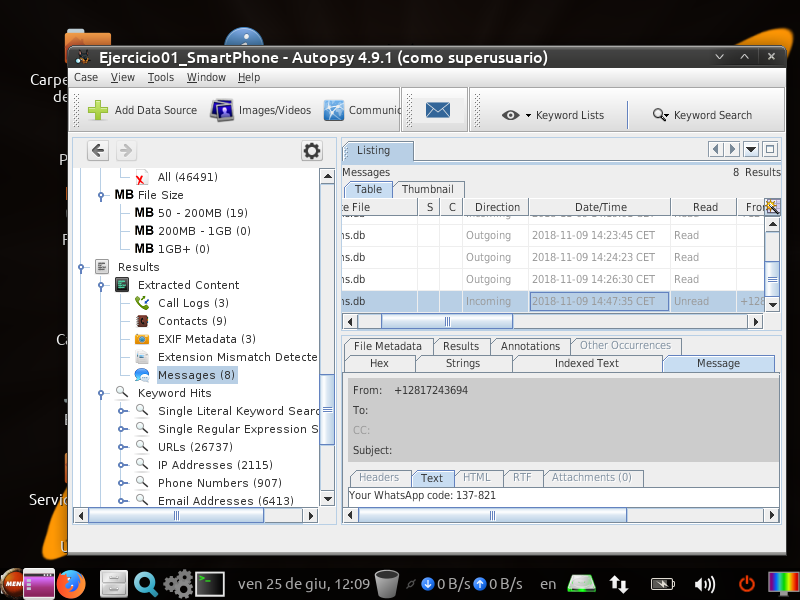
\includegraphics[scale=0.7]{e1-25.png}
\end{figure}

aa) El módulo de búsqueda de cadenas detectó 6413 direcciones de email.

\begin{figure}[H]
    \caption{Ejercicio 1: Direcciones de email}
    \centering
    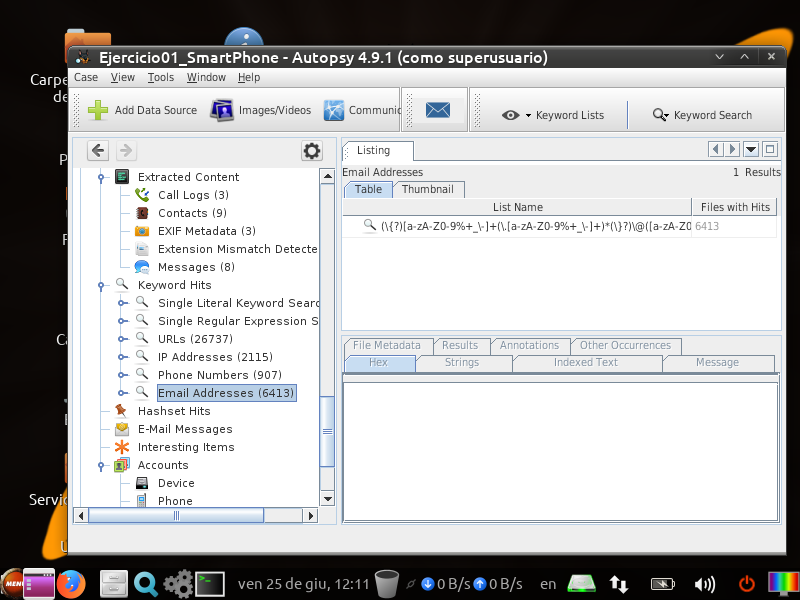
\includegraphics[scale=0.7]{e1-26.png}
\end{figure}

bb) Se puede buscar en el apartado Views por tipo MIME, se observa que hay un único fichero gif detectado, llamado \textit{homer.gif}.

\begin{figure}[H]
    \caption{Ejercicio 1: Ficheros gif}
    \centering
    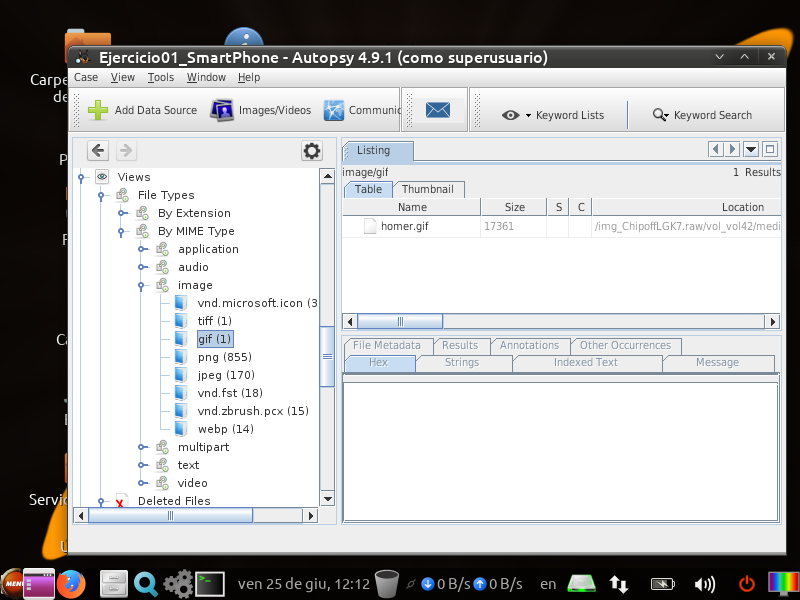
\includegraphics[scale=0.7]{e1-27.png}
\end{figure}

cc) Se muestra a continuación una captura del fichero \textit{homer.gif}.

\begin{figure}[H]
    \caption{Ejercicio 1: \textit{homer.gif}}
    \centering
    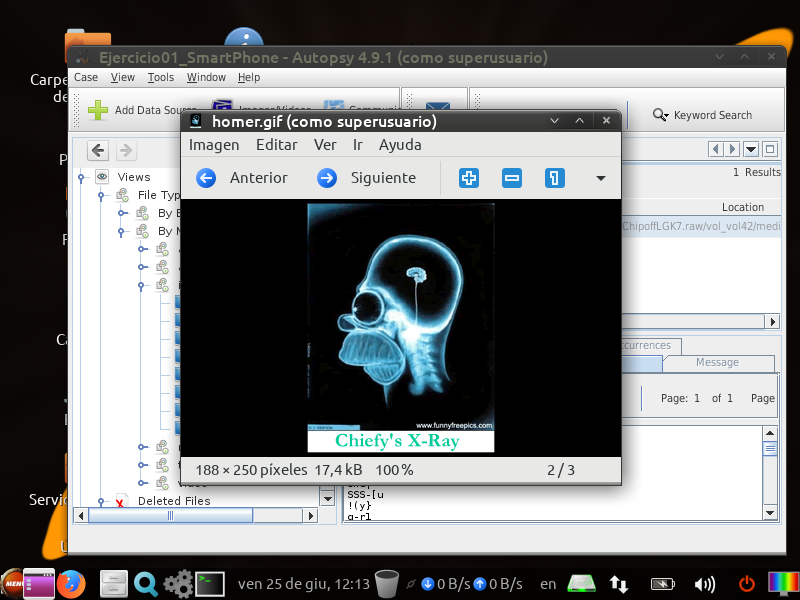
\includegraphics[scale=0.7]{e1-28.png}
\end{figure}

dd) Se busca entre las subcarpetas de \textit{/userdata/data} (en la partición 42) las posibles redes sociales que maneja el usuario. Se encuentran \textit{Facebook}, \textit{Instagram}, \textit{LinkedIn}, \textit{Pinterest}, \textit{Snapchat}, \textit{Twitter}, \textit{Whatsapp} y \textit{Youtube}.

\begin{figure}[H]
    \caption{Ejercicio 1: \textit{/userdata/data}}
    \centering
    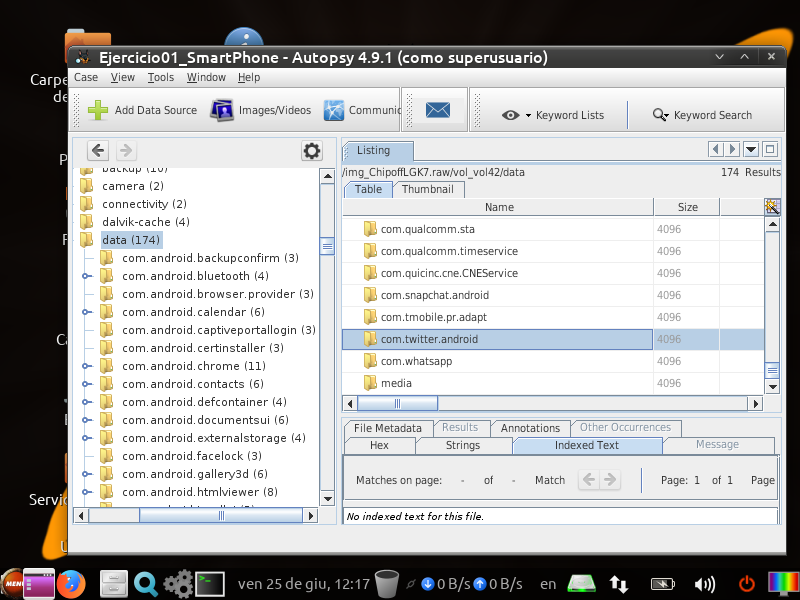
\includegraphics[scale=0.7]{e1-29.png}
\end{figure}

ee) Se extrae el fichero \textit{packages.xml}, encontrado en la carpeta \textit{/system} del volumen 42.

\begin{figure}[H]
    \caption{Ejercicio 1: \textit{/system}}
    \centering
    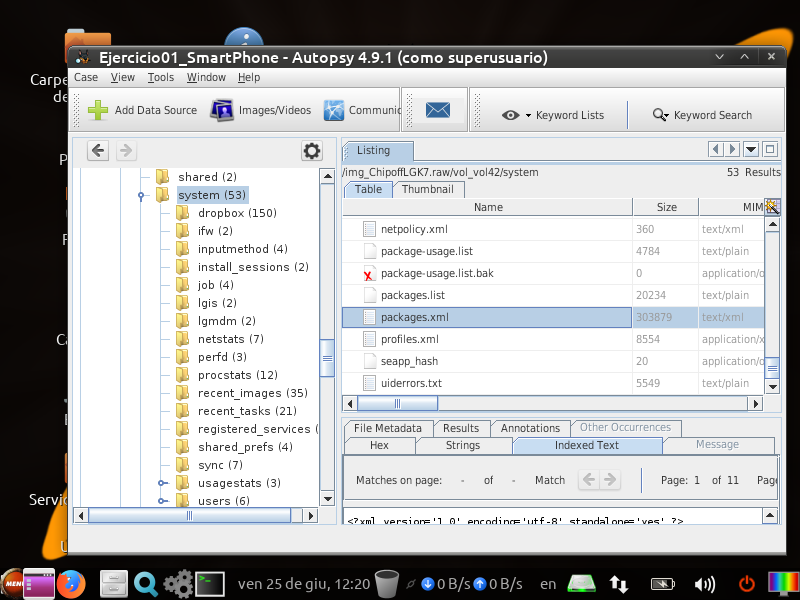
\includegraphics[scale=0.7]{e1-30.png}
\end{figure}

ff) Se muestran a continuación las líneas de los permisos de \textit{Whatsapp} en el editor Vim.

\begin{figure}[H]
    \caption{Ejercicio 1: Permisos Whatsapp}
    \centering
    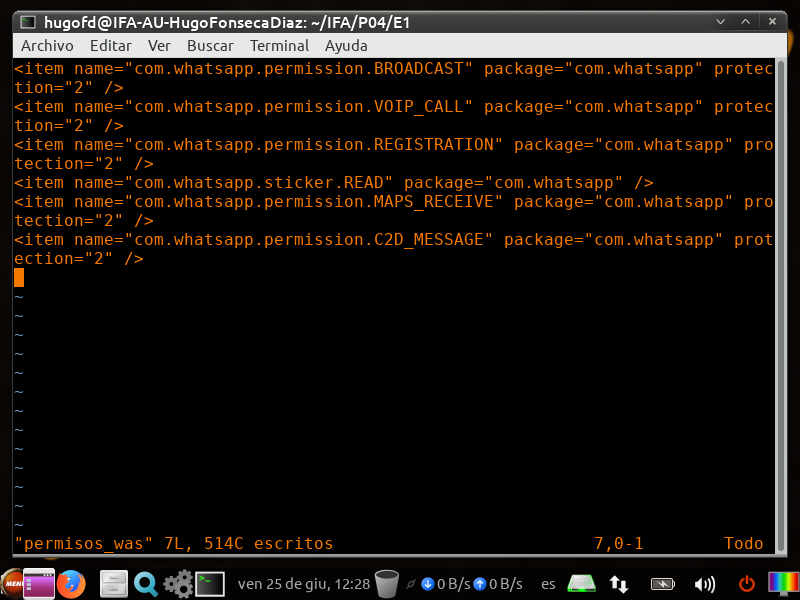
\includegraphics[scale=0.7]{e1-31.png}
\end{figure}

gg) El instalador de \textit{Whatsapp} se encuentra en \textit{com.android.vending}, dentro de la carpeta \textit{/data}.

hh) Hay seis cuentas asociadas.

\begin{figure}[H]
    \caption{Ejercicio 1: \textit{Accounts.db} - Tabla \textit{accounts}}
    \centering
    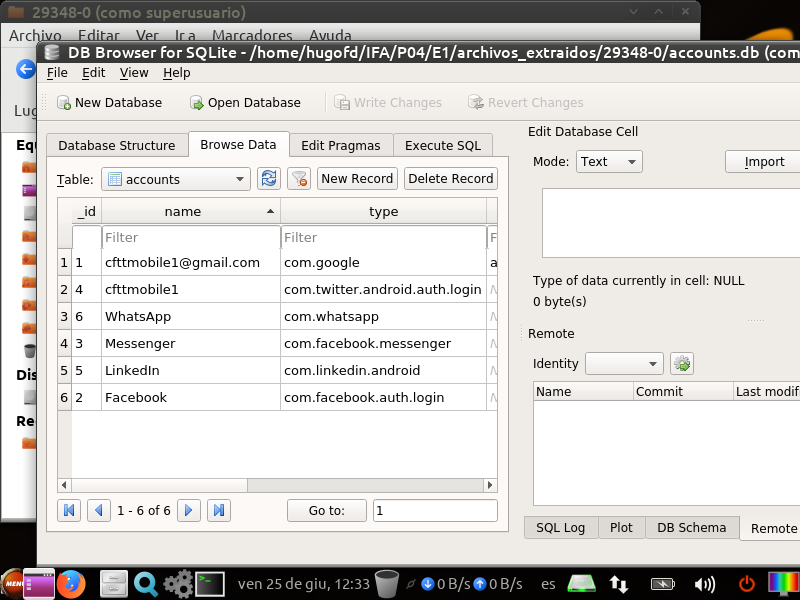
\includegraphics[scale=0.7]{e1-32.png}
\end{figure}

ii) La cuenta de Google es \textit{cfttmobile1@gmail.com}. Puede observarse en la anterior captura.

jj) Puede observarse la contraseña hasheada en la siguiente captura.

\begin{figure}[H]
    \caption{Ejercicio 1: Contraseña hasheada}
    \centering
    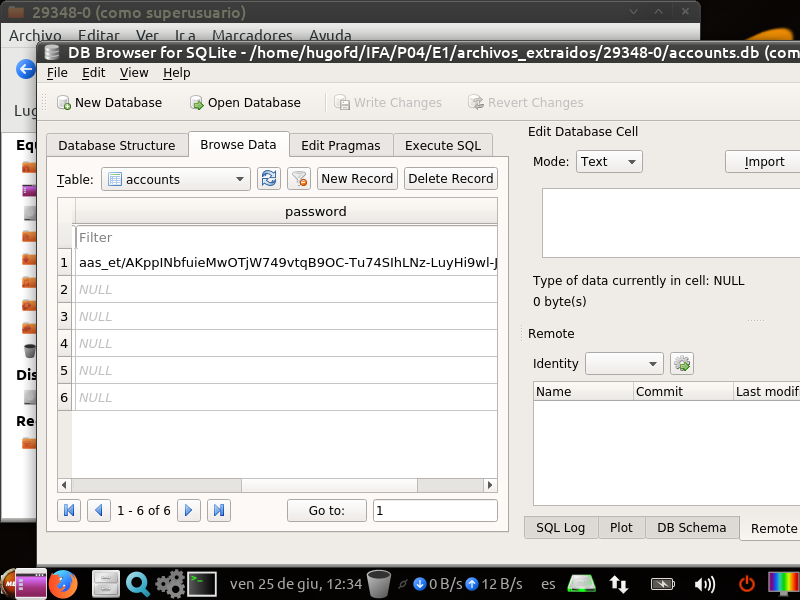
\includegraphics[scale=0.7]{e1-33.png}
\end{figure}



% Bibliografía
\begin{thebibliography}{8}
\end{thebibliography}

\end{document}




